\documentclass[10pt, letterpaper]{article}

%% Language and font encodings
\usepackage[english]{babel}
\usepackage[utf8x]{inputenc}
\usepackage[T1]{fontenc}

% definign page geometry
\usepackage[a4paper, top=2cm, bottom=2cm, left=3cm, right=2cm, marginparwidth=1.75cm]{geometry}
\usepackage{caption, subcaption}
\captionsetup[table]{skip=10pt}
\captionsetup[subfigure]{justification=justified,singlelinecheck=false}

% Useful packages
\usepackage{amsmath, graphicx, natbib, multicol, booktabs}
\usepackage[colorinlistoftodos]{todonotes}
\usepackage[colorlinks=true, allcolors=blue]{hyperref}
\bibliographystyle{unsrt}

% section sizing
\usepackage{titlesec}
\titleformat*{\subsection}{\normalsize\bfseries}

% Title
\title{
    \usefont{OT1}{bch}{b}{n}
    \normalfont \normalsize \textsc{STEM Fellowship Big Data Challenge 2020} \\ [10pt]
    \huge Deep learning transcriptomic model for prediction of pan-drug chemotherapeutic sensitivity \\
}
\selectlanguage{english}
\usepackage{authblk}
\author[1]{Eddie Guo}
\author[2]{Mehul Gupta}
\author[1]{Pouria Torabi}
\author[2]{Sunand Kannappan}
\affil[1]{University of Alberta}
\affil[2]{University of Calgary}

% drawing neural network
\usepackage{tikz}
\usetikzlibrary{shapes, arrows}
\tikzset{
  every neuron/.style={
    circle,
    draw,
    minimum size=1cm
  },
  neuron missing/.style={
    draw=none, 
    scale=3,
    text height=0.333cm,
    execute at begin node=\color{black}$\vdots$
  },
}

\usepackage{ifthen}
\newcommand{\foo}[1]{%
  \ifthenelse{\equal{#1}{missing}}
    {}
    {$H^{(1)}_{\l}$}
}

\newcommand{\hehe}[1]{%
  \ifthenelse{\equal{#1}{missing}}
    {}
    {$H^{(2)}_{\l}$}
}

\newcommand{\hehetwo}[1]{%
  \ifthenelse{\equal{#1}{missing}}
    {}
    {$H^{(3)}_{\l}$}
}

\newcommand{\hehethree}[1]{%
  \ifthenelse{\equal{#1}{missing}}
    {}
    {$H^{(4)}_{\l}$}
}

\newcommand{\hehefour}[1]{%
	\ifthenelse{\equal{#1}{missing}}
	{}
	{$H^{(5)}_{\l}$}
}

\newcommand{\lmao}[1]{%
  \ifthenelse{\equal{#1}{missing}}
    {}
    {$I_{\l}$}
}

% define flowchart styles
\tikzstyle{block} = [rectangle, rounded corners, minimum height=3em, draw=black, inner sep=1em]
\tikzstyle[line] = [draw, -latex']
\tikzstyle{stop} = [rectangle, rounded corners, minimum width=2cm, minimum height=0.5cm,text centered, draw=black]
\tikzstyle{arrow} = [thick,->,>=stealth]

\frenchspacing
\setlength{\parskip}{0em}


\begin{document}
\maketitle


% Abstract
\begin{abstract}
	Emerging precision oncology studies have yet to generate a predictive biomarker that utilizes gene expression profiles to stratify tumours into similar pan-drug sensitivity profiles. This development would allow for the identification of candidate drugs for treatments that maximize therapeutic response and minimize cytotoxic burden. As such, this study utilized cell line sensitivity and molecular profiling data to generate a combinatorial gene expression predictive biomarker via feature selection and a deep learning model. A cohort of cell line gene expression data from Genomics of Drug Sensitivity in Cancer (GDSC) was clustered into two response groups. Cell line response groups showed a significant difference in pan-drug chemotherapeutic sensitivity. Due to the high dimensional nature of the microarray data, the Boruta feature selection algorithm was used to identify genes with the highest predictive value. The feature space was reduced to 300 genes; functional profiling was enriched primarily for the focal adhesion, ECM-receptor and proteoglycan interaction pathways. Using the selected genes, a deep learning neural network architecture was developed to predict response groups. It was determined that a 10 hidden layer neural network was optimal for the dataset; following hyperparameter tuning and 5-fold cross-validation, the model showed a predictive accuracy of 95.4\% (AUC = 0.913 $\pm$ 0.049).  This validates the postulate that cell lines with similar gene expression profiles present similar pan-drug chemotherapeutic sensitivity, and it suggests the potential utility of similar combinatorial biomarkers for the selection of potent candidate drugs. \vspace{1em}

	% Keywords
	\noindent {\textbf{Keywords}\\
		clustering, neural network, transcriptomics, chemotherapeutic response, combinatorial biomarker, molecular profile, therapeutic sensitivity, cancer}
\end{abstract} \vspace{1em}

\begin{multicols*}{2}
% Introduction
\section{Introduction}
With the advent of high-throughput sequencing technology, precision oncology approaches have utilized molecular characteristics of tumours to inform clinical decision-making, including choice of chemotherapeutic regimen \cite{drugml, patient_resps}. The major focus of these approaches has been the development of targeted therapeutics, which are selective for specific genetic aberrations and expression profiles. Although these approaches may be successful for inducing tumour response, tumours are more likely to gain resistance to therapies with specific targets \cite{small_mol}. Moreover, not all tumours present with targetable features \cite{small_mol}.

Emerging precision oncology approaches have begun to utilize high-throughput technology to potentiate the usage of conventional and less-targeted chemotherapy. Given that many of these less-targeted and consequently more cytotoxic chemotherapies have broad activity, the primary determinants of chemotherapeutic selection include cancer type and certain molecular markers \cite{adverse}. Nevertheless, it is well established that tumour sensitivity to chemotherapy is heterogeneous both between and within cancer types, which results in a subset of patients that fail to respond to conventional chemotherapy regimens while being subjected to significant side effect burden \cite{adjuvant}. Given that evidence suggests that gene expression can mediate drug response, recent advances have utilized individual and combinatorial gene expression biomarkers to develop predictors of tumour sensitivity to chemotherapeutic compounds \cite{integrated}.

While previous studies have developed predictive biomarkers for specific drugs, the utility of these biomarkers is limited to particular patients and clinical contexts \cite{drug_sense}. That is, these studies are limited in terms of clinical generalizability to different chemotherapeutic regimens. However, a pan-drug predictive biomarker may provide significant clinical utility in the selection of candidate therapies for particular patients. Such a biomarker could be developed if tumours with similar expression have similar drug responses across all chemotherapies, with few exceptions. The availability of pan-cancer cell line databases with \textit{in vitro} drug sensitivity analyses along with accompanying gene expression profiling provides an ideal model for such analyses \cite{gdsc}. However, the majority of previous drug sensitivity predictive biomarkers built on cell line databases have utilized classical machine learning combinatorial techniques, which fail to capture the dimensionality of available transcriptomic data. Furthermore, advanced deep learning algorithmic approaches that are capable of handling such dimensionality often fail to allow interpretability, and consequently require transcriptomic data that is clinically infeasible \cite{ml_oncol}. Thus, deep learning approaches should minimize the number of transcriptomic features selected to maximize both the accuracy and interpretability of such predictive biomarkers.

Here we set out to generate a deep learning transcriptomic model for the prediction of pan-drug chemotherapeutic sensitivity across cell lines of all cancer types. If successful, this would demonstrate that gene expression influences chemotherapeutic response across most drugs and further motivate future studies into the development of clinically applicable predictors of candidate chemotherapeutics for tumours of a specific gene expression profile.

Following unsupervised clustering of cell lines into therapeutic response groups with similar pan-drug sensitivity, we show that conventional clinical criteria fail to stratify cell lines by therapeutic response. We utilize a biologically agnostic feature selection algorithm to iteratively select and identify a subset of 300 relevant genes predictive of chemotherapeutic sensitivity. We then develop a deep learning model from the selected genes utilizing neural networks, which showcases a strong predictive ability across pan-cancer cell lines.


% Materials and Methods
\section{Methods}

We developed a deep learning model to accurately classify cancer cell lines into therapeutic response groups using data from the Genomics of Drug Sensitivity in Cancer (GDSC) consortium. Following data collection and curation, we utilized unsupervised clustering algorithms to define two groups based on chemotherapeutic response. Next, we employed a biologically agnostic feature selection algorithm, Boruta, to select statistically relevant genes for our neural network. These transcriptomic features were fed into a neural network that classifies patients into therapeutic response groups as defined by the clustering algorithms. The neural network architecture was optimized using a grid search and evaluated using 5-fold cross-validation See Fig. \ref{fig:pipeline} for an overview of the data analysis pipeline.


\subsection{Determining pan-cancer therapeutic response cohorts}
To better understand the impact and predictive ability of transcriptomic dysregulation in chemotherapeutic response, a pan-cancer cohort of cell line and associated therapeutic sensitivity data were obtained from the GDSC database. This database includes 1,110 cell lines from various tumour types, and is thought to represent a relatively comprehensive pan-cancer dataset. In addition, the acquired dataset contained therapeutic efficacy information in the form of half-maximal inhibitory concentration (IC$_{50}$) values for 251 chemotherapies. These values correspond to the minimal concentration of therapeutic required to induce cell death in 50\% of the cultured cells, with lower values being associated with improved drug efficacy. The data was used to generate a matrix with cell line and accompanying therapeutic information. This dataset was filtered to exclude therapies with less than 80\% of data for all cell lines, followed by the exclusion of cell lines lacking response data for the drugs retained in the first step.


% flowchart figure
\begin{figure*}[!ht]
    \centering
    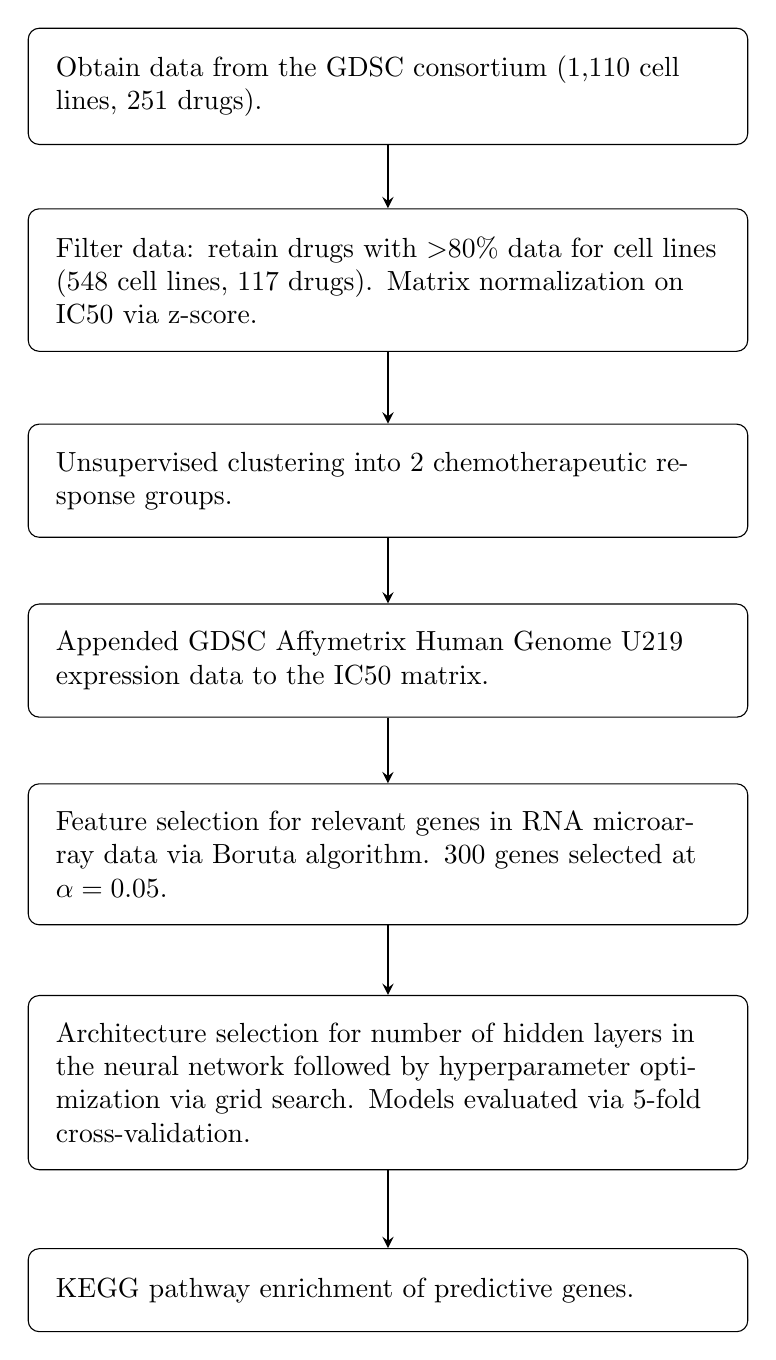
\begin{tikzpicture}[node distance=6em, auto]
        % blocks
        \node [block, text width=24em] (init) {Obtain data from the GDSC consortium (1,110 cell lines, 251 drugs).};
        \node [block, below of=init, text width=24em, yshift=-1em] (process) {Filter data: retain drugs with $>$80\% data for cell lines (548 cell lines, 117 drugs). Matrix normalization on IC50 via z-score.};
        \node [block, below of=process, text width=24em, yshift=-1.25em] (kmeans) {Unsupervised clustering into 2 chemotherapeutic response groups.};
        \node [block, below of=kmeans, text width=24em, yshift=-0.5em] (append) {Appended GDSC Affymetrix Human Genome U219 expression data to the IC50 matrix.};
        \node [block, below of=append, text width=24em, yshift=-1em] (feat) {Feature selection for relevant genes in RNA microarray data via Boruta algorithm. 300 genes selected at $\alpha=0.05$.};
        \node [block, below of=feat, text width=24em, yshift=-2.25em] (neural) {Architecture selection for number of hidden layers in the neural network followed by hyperparameter optimization via grid search. Models evaluated via 5-fold cross-validation.};
        \node [block, below of=neural, text width=24em, yshift=-1.5em] (annot) {KEGG pathway enrichment of predictive genes.};

        % arrows
        \draw [arrow] (init) -- (process);
        \draw [arrow] (process) -- (kmeans);
        \draw [arrow] (kmeans) -- (append);
        \draw [arrow] (append) -- (feat);
        \draw [arrow] (feat) -- (neural);
        \draw [arrow] (neural) -- (annot);
    \end{tikzpicture}
    \caption{Summary of the data analysis pipeline.}
    \label{fig:pipeline}
\end{figure*}


\subsection{Identification of pan-cancer therapeutic response cohorts}
Cell line therapeutic sensitivity matrices were used to evaluate whether conventional clinical criteria could separate patients into previously-defined chemotherapeutic response groups. These conventional clinical criteria included anatomic location and solid versus non-solid tumour status, as well as broadly applicable molecular markers -- TP53 and KRAS mutation status \cite{colorectal, gi, lung, breast}. Cell lines were separated into subgroups based on these criteria and visualized to determine whether these criteria effectively clustered response groups.

Following evaluation of existing classifiers, we attempted to create defined cell line clusters using observed chemotherapeutic response of the pan-cancer cell line samples. We developed a Euclidean distance matrix for the retained cell lines based on their pan-chemotherapy response. This matrix was then used to identify the minimum number of clusters capable of representing the therapeutic heterogeneity identified across the cancer cell lines while maintaining significant inter-cluster distance. Following this, k-means clustering was utilized to assign cell line candidates to appropriate therapeutic response cohorts. Generalized differences in chemotherapeutic efficacy between cohorts were visualized using a heatmap generated by the pheatmap package \cite{pheatmap} in R. Separation between clusters was also visualized using principal component analysis with the factoextra package \cite{factoextra} in R. Following the identification of defined clusters, differences in therapeutic efficacy between the identified cohorts were evaluated. Mann-Whitney U tests were utilized to compare IC$_{50}$ values between the groups. False discovery rate (FDR) correction was utilized to correct for multiple comparisons.


% PCA figures
\begin{figure*}[!ht]
	\centering
    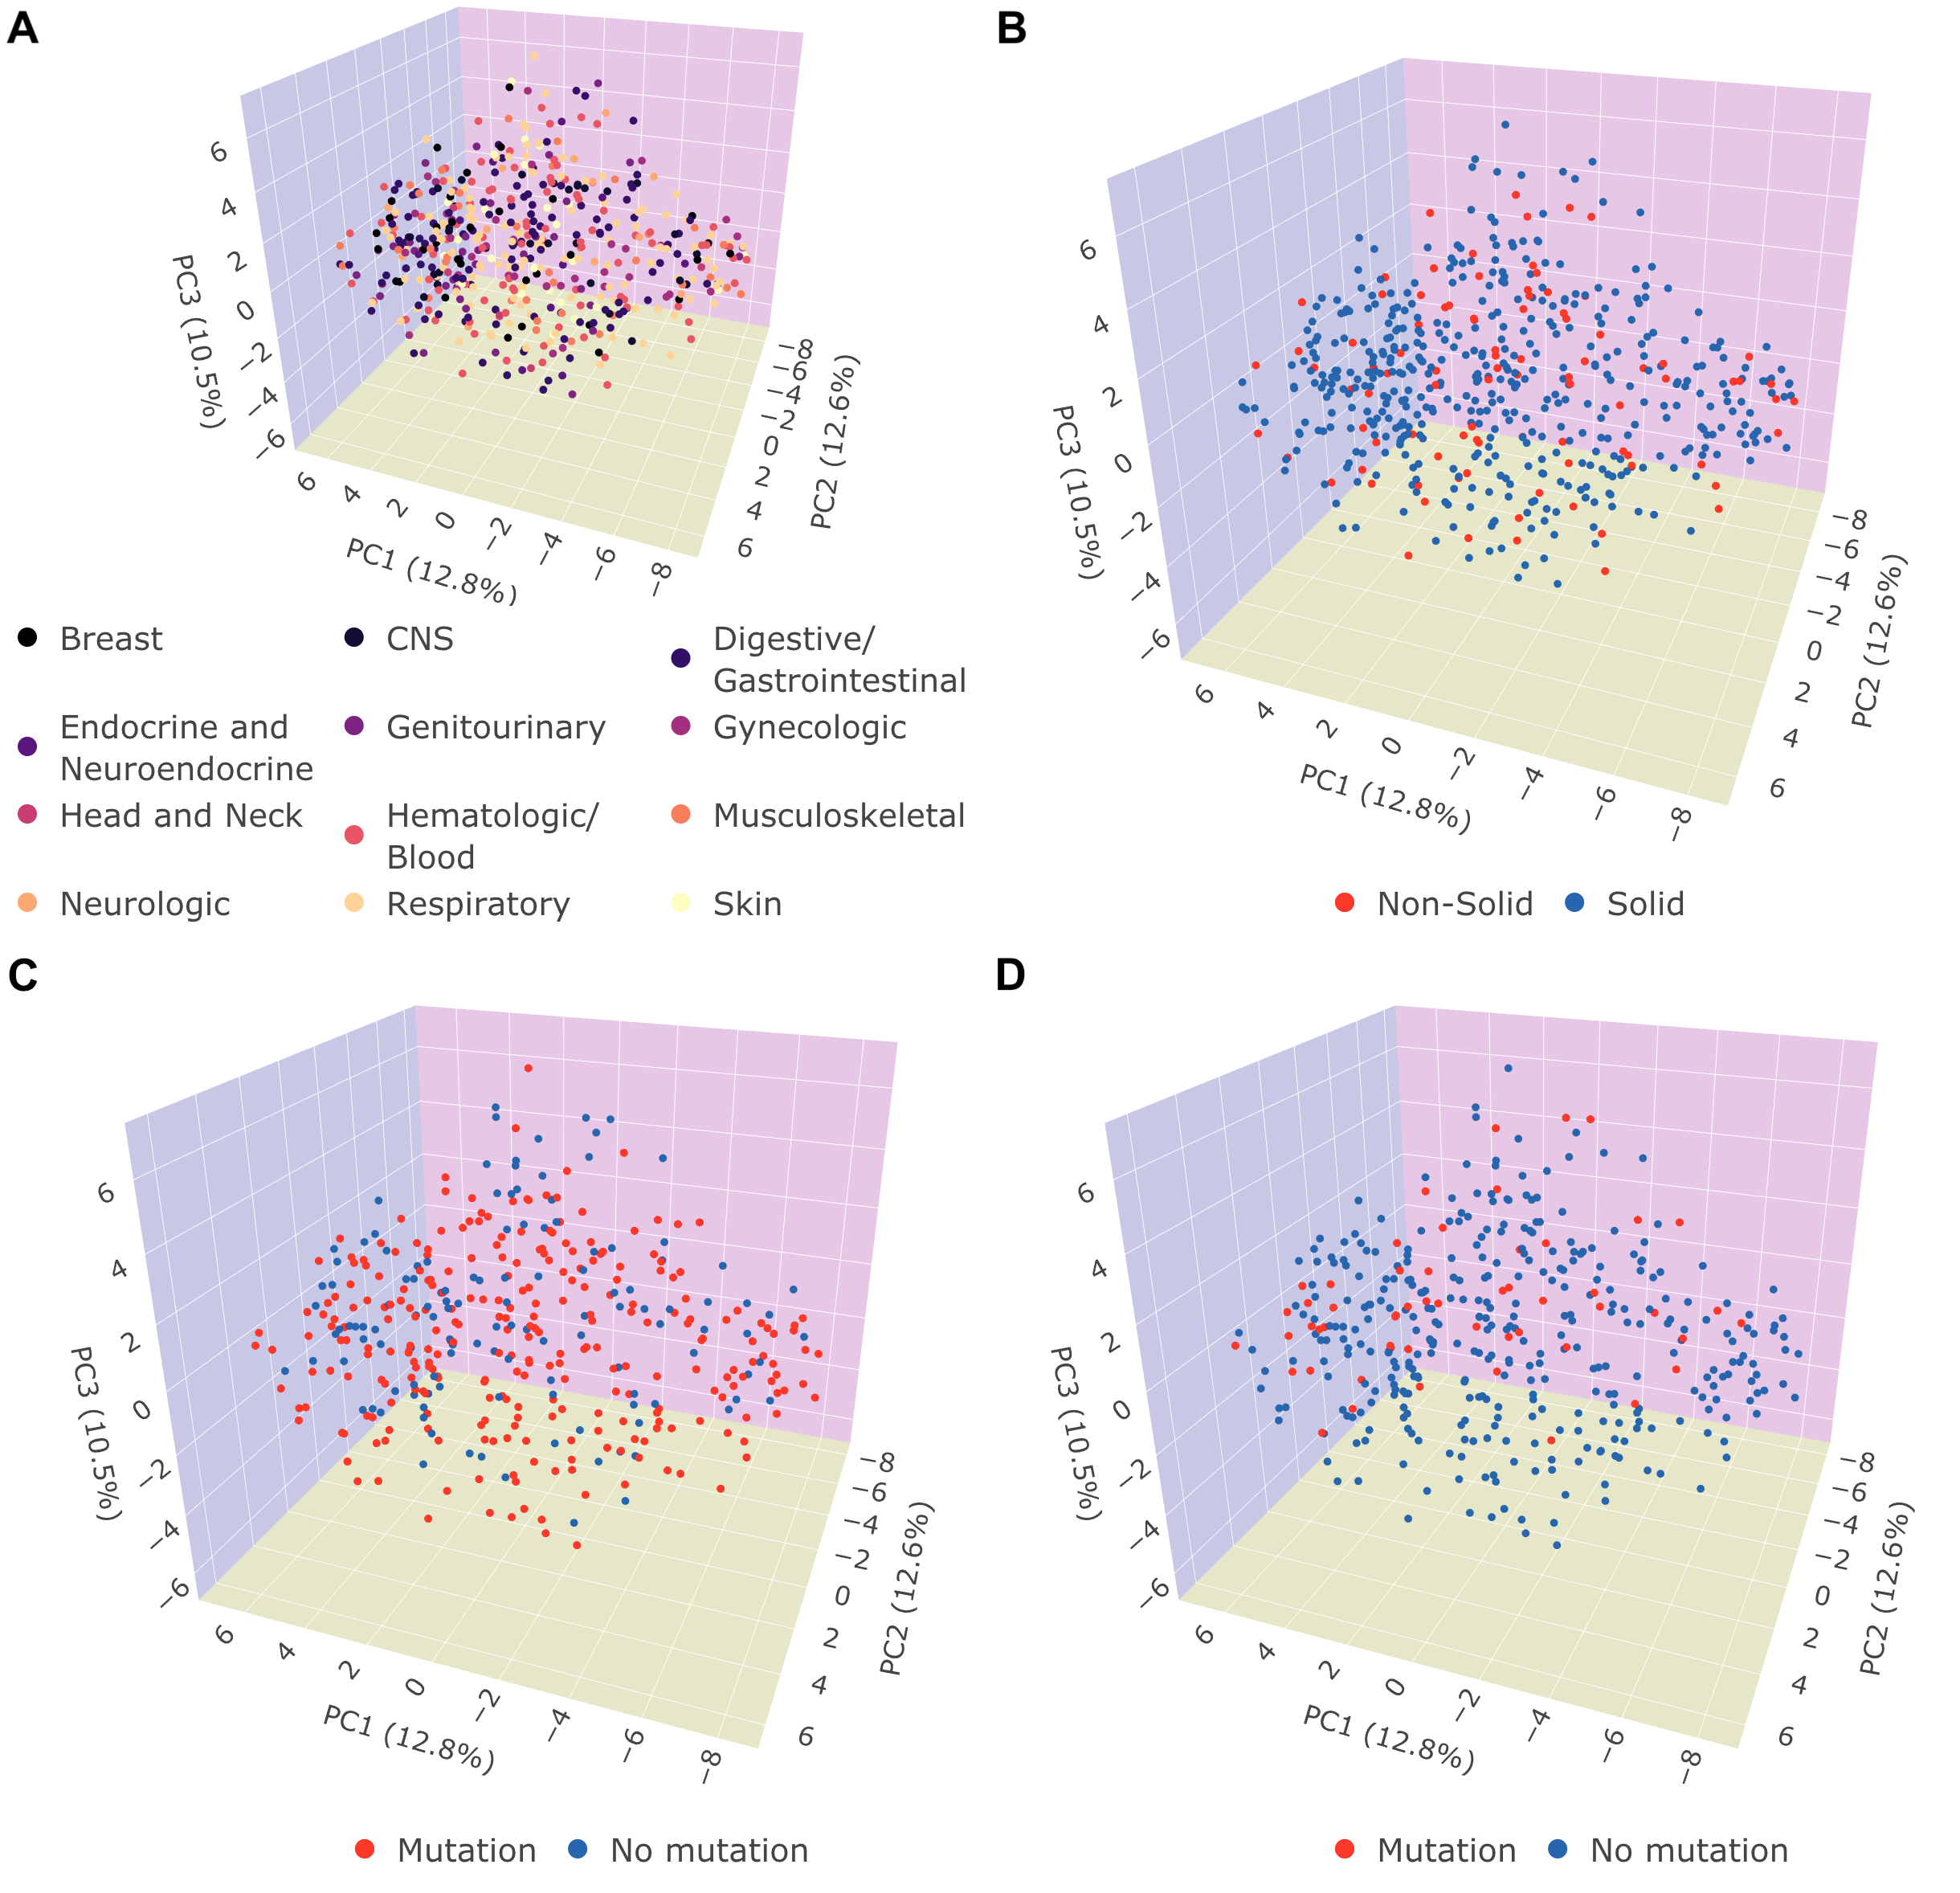
\includegraphics[width=\textwidth]{Figures/initial_pca.png}

	\caption{Principal component analysis of pan-cancer cell line therapeutic efficacy, generated from IC$_{50}$ values of all available chemotherapeutics.The horizontal axis shows the first principal component, the vertical axis the second component. Cell lines are visualized based on major cancer type classifications, including (\textbf{A}) body system of tumour and (\textbf{B}) solid vs. non-solid tumour status. Cell lines were also visualized on major molecular markers, including (\textbf{C}) TP53 mutation status, and (\textbf{D}) KRAS mutation status.}
	\label{fig:overall_pca}
\end{figure*}


% clustering figure
\begin{figure*}[!ht]
    \centering
    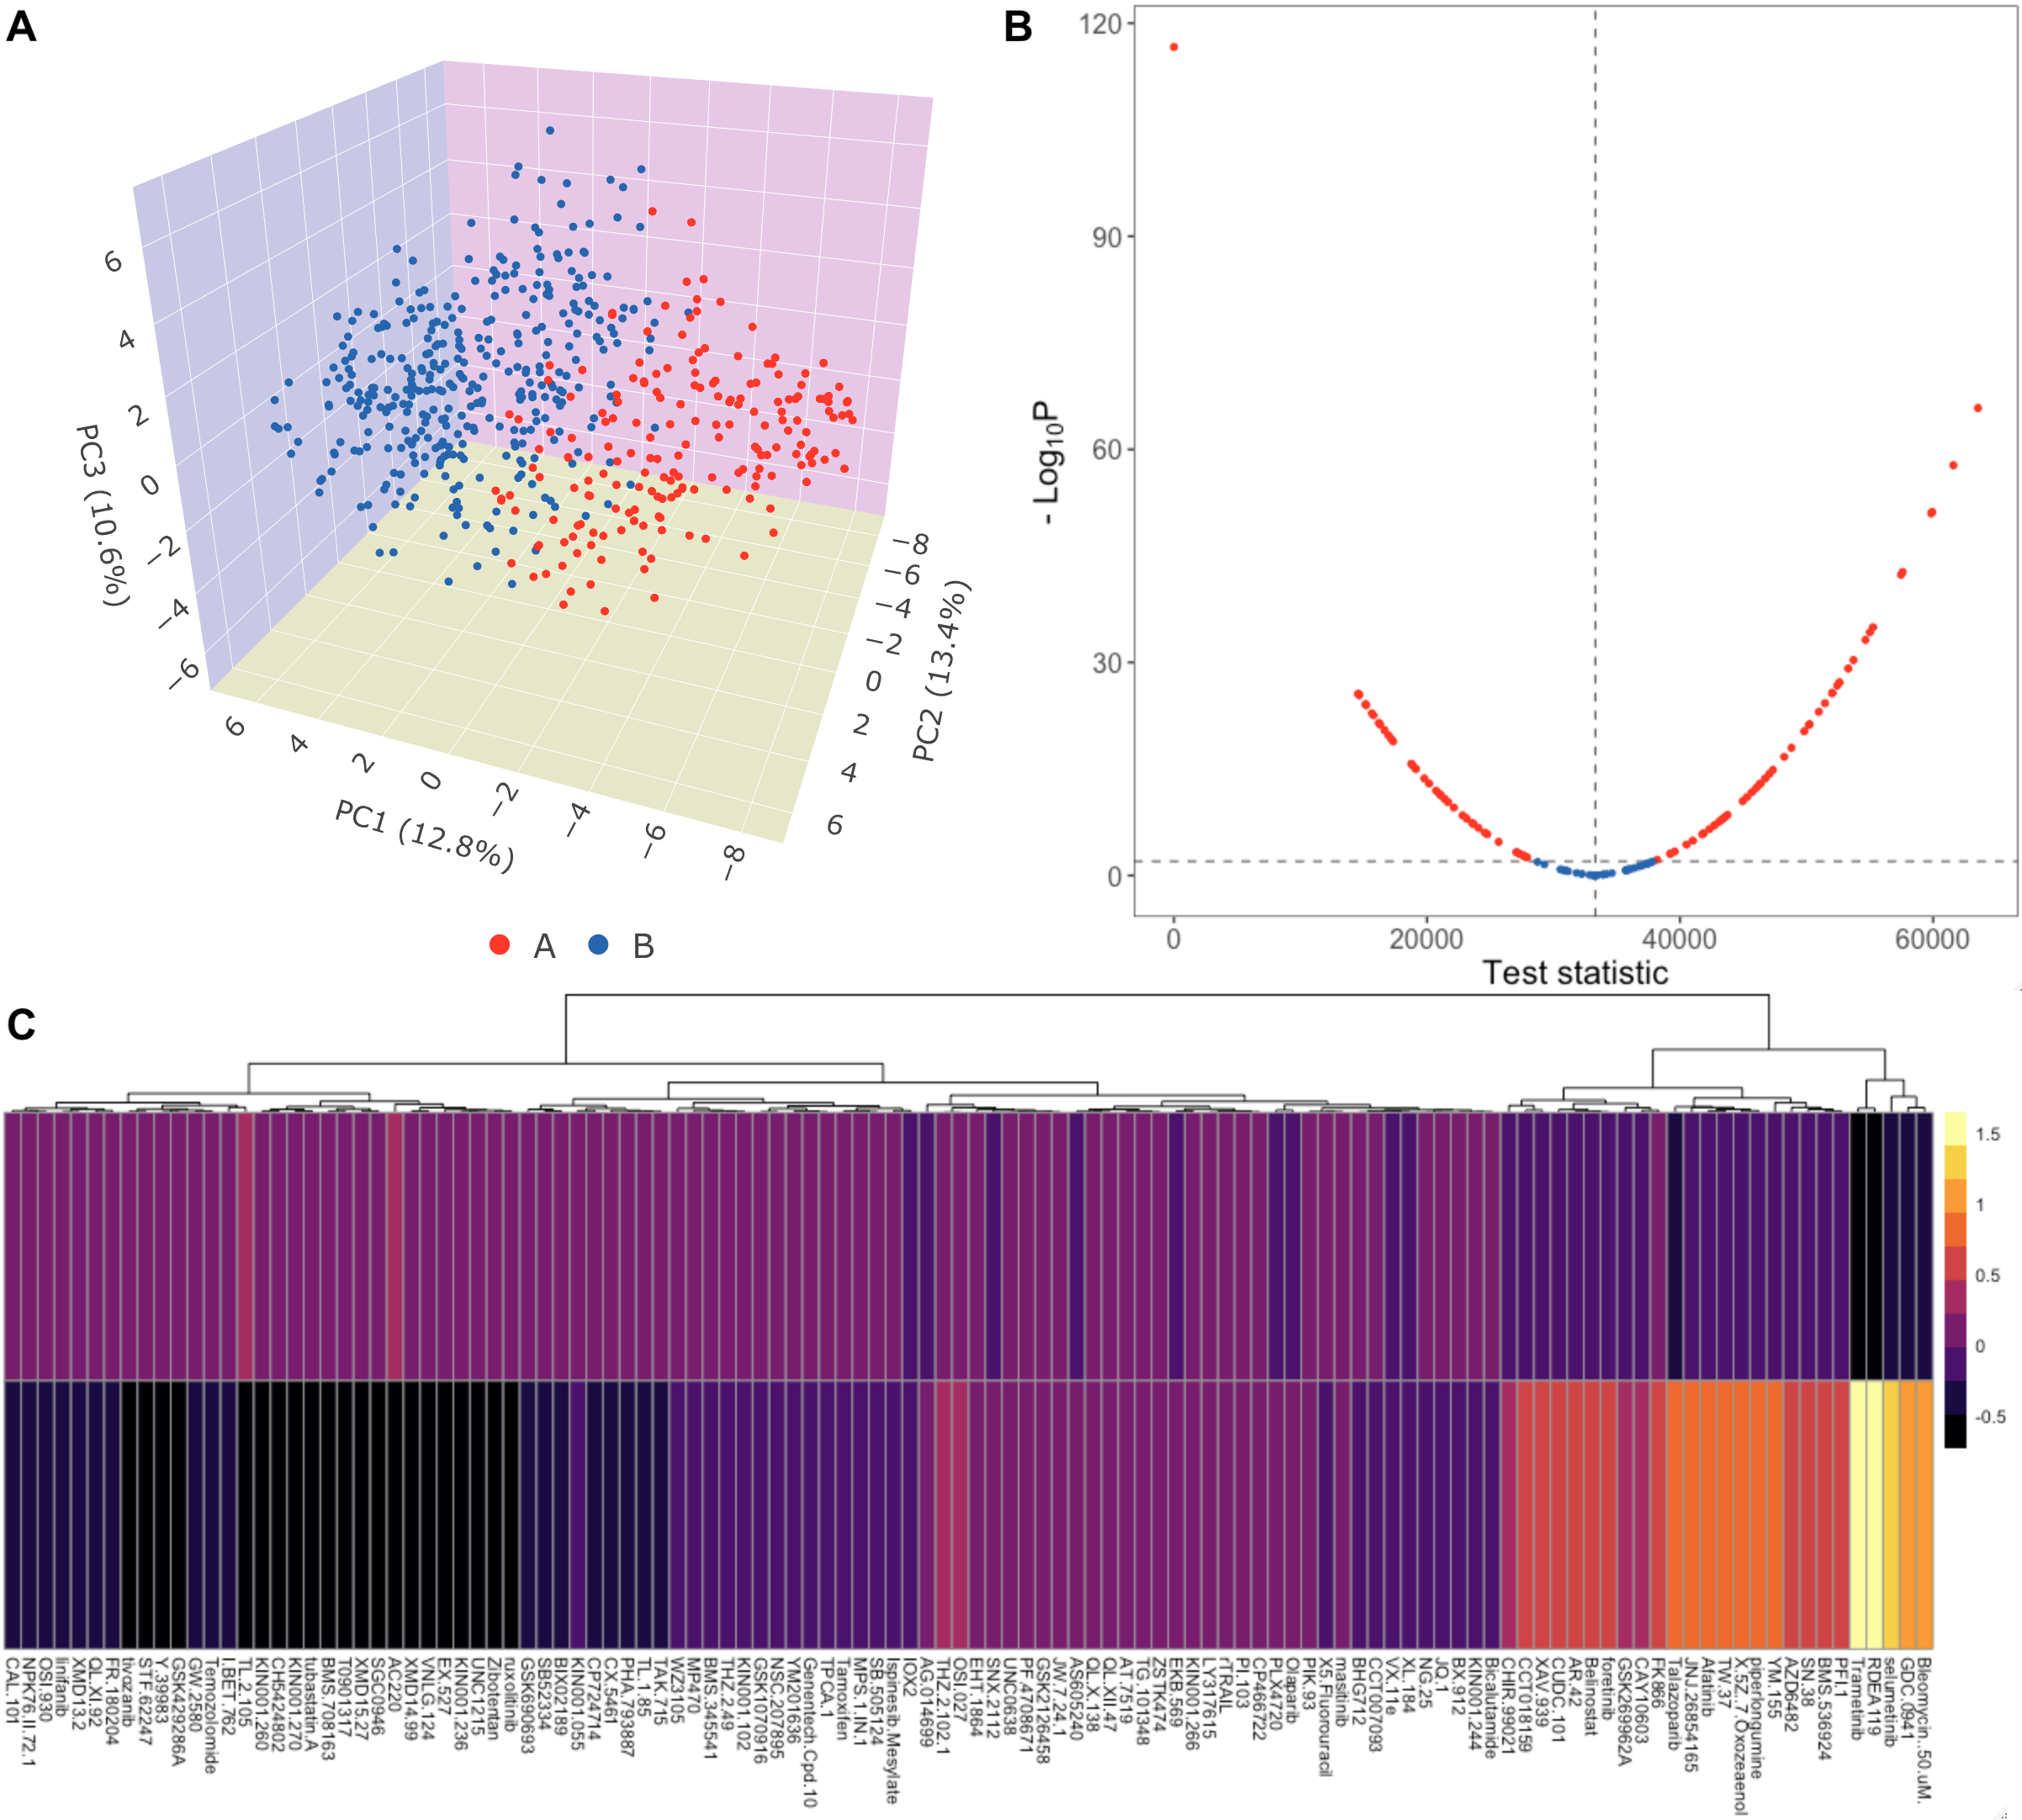
\includegraphics[width=\textwidth]{Figures/clustering.png}

    \caption{(\textbf{A}) Principal component analysis of pan-cancer cell line therapeutic efficacy, generated from IC$_{50}$ values of all available chemotherapeutics. The horizontal axis shows the first principal component, the vertical axis the second component. The two identified therapeutic response clusters are indicated in red and blue respectively. (\textbf{B}) Volcano plot identifying chemotherapeutics with significantly different IC$_{50}$ values between therapeutic response clusters. Drugs identified in red meet the criteria for significance (FDR adjusted $p<0.05$). (\textbf{C}) Heatmap of therapeutic IC$_{50}$ for the two identified therapeutic response clusters. Columns represent individual chemotherapies and are clustered according to Euclidean distance. Colours range from yellow to black, with a shift toward the latter indicating increased efficacy of the corresponding chemotherapeutic.}
    \label{fig:clustering}
\end{figure*}


\subsection{Feature Selection with Boruta}
In order to develop a transcriptomic model predictive of therapeutic response clusters, we retrieved expression data quantified by the GDSC consortium using the Affymetrix U219 microarray for each candidate cell line. Here, minimally processed CEL files were obtained from ArrayExpress (ascension number E-MTAB-3610) and processed using the affy package \cite{affy} in R. The resulting normalized expression matrix for candidate cell lines was then merged with the existing dataset. This addition resulted in the loss of 7 cell lines (2 from cluster A and 5 from cluster B), resulting in the inclusion of 541 cell lines in model generation. The microarray dataset quantified the expression of 16,382 genes; a model developed from this large feature space is likely to exhibit high multicollinearity and subsequently overfit, compromising the generalizability of the model. In addition, the large feature space limits the efficiency of various feature selection algorithms\footnote{For example, univariate selection or recursive feature elimination.} as well as training and optimizing neural networks. We addressed these issues with the Boruta feature selection algorithm using the BorutaPy package \cite{liu} in Python 3. Boruta is a feature selection algorithm based on Random Forest classification which iteratively removes features that are statistically less significant than a shuffled version of the same feature \cite{kursa}


% neural net evaluation figure
\begin{figure*}[!ht]
    \centering
    \begin{subfigure}[t]{\textwidth}
        \centering
        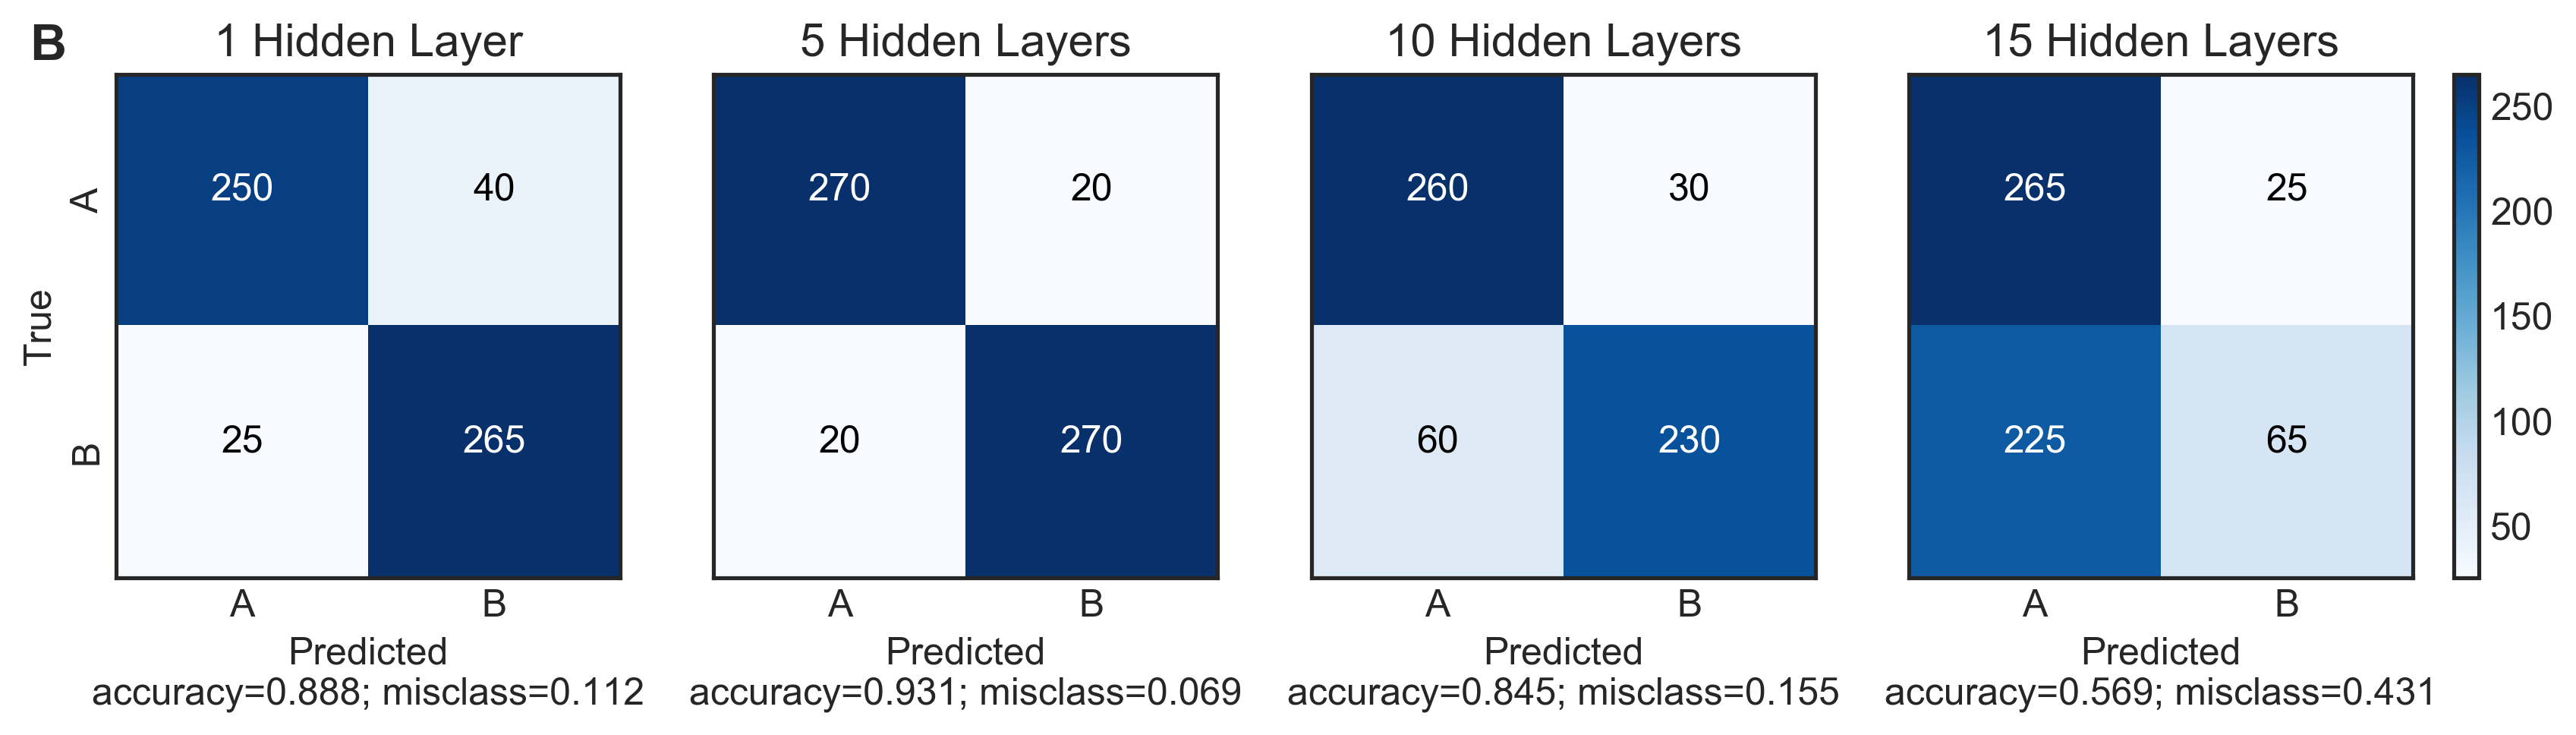
\includegraphics[width=\textwidth]{Figures/confusion_matrix/cm_combined.png}
    \end{subfigure}

    \begin{subfigure}[t]{\textwidth}
        \centering
        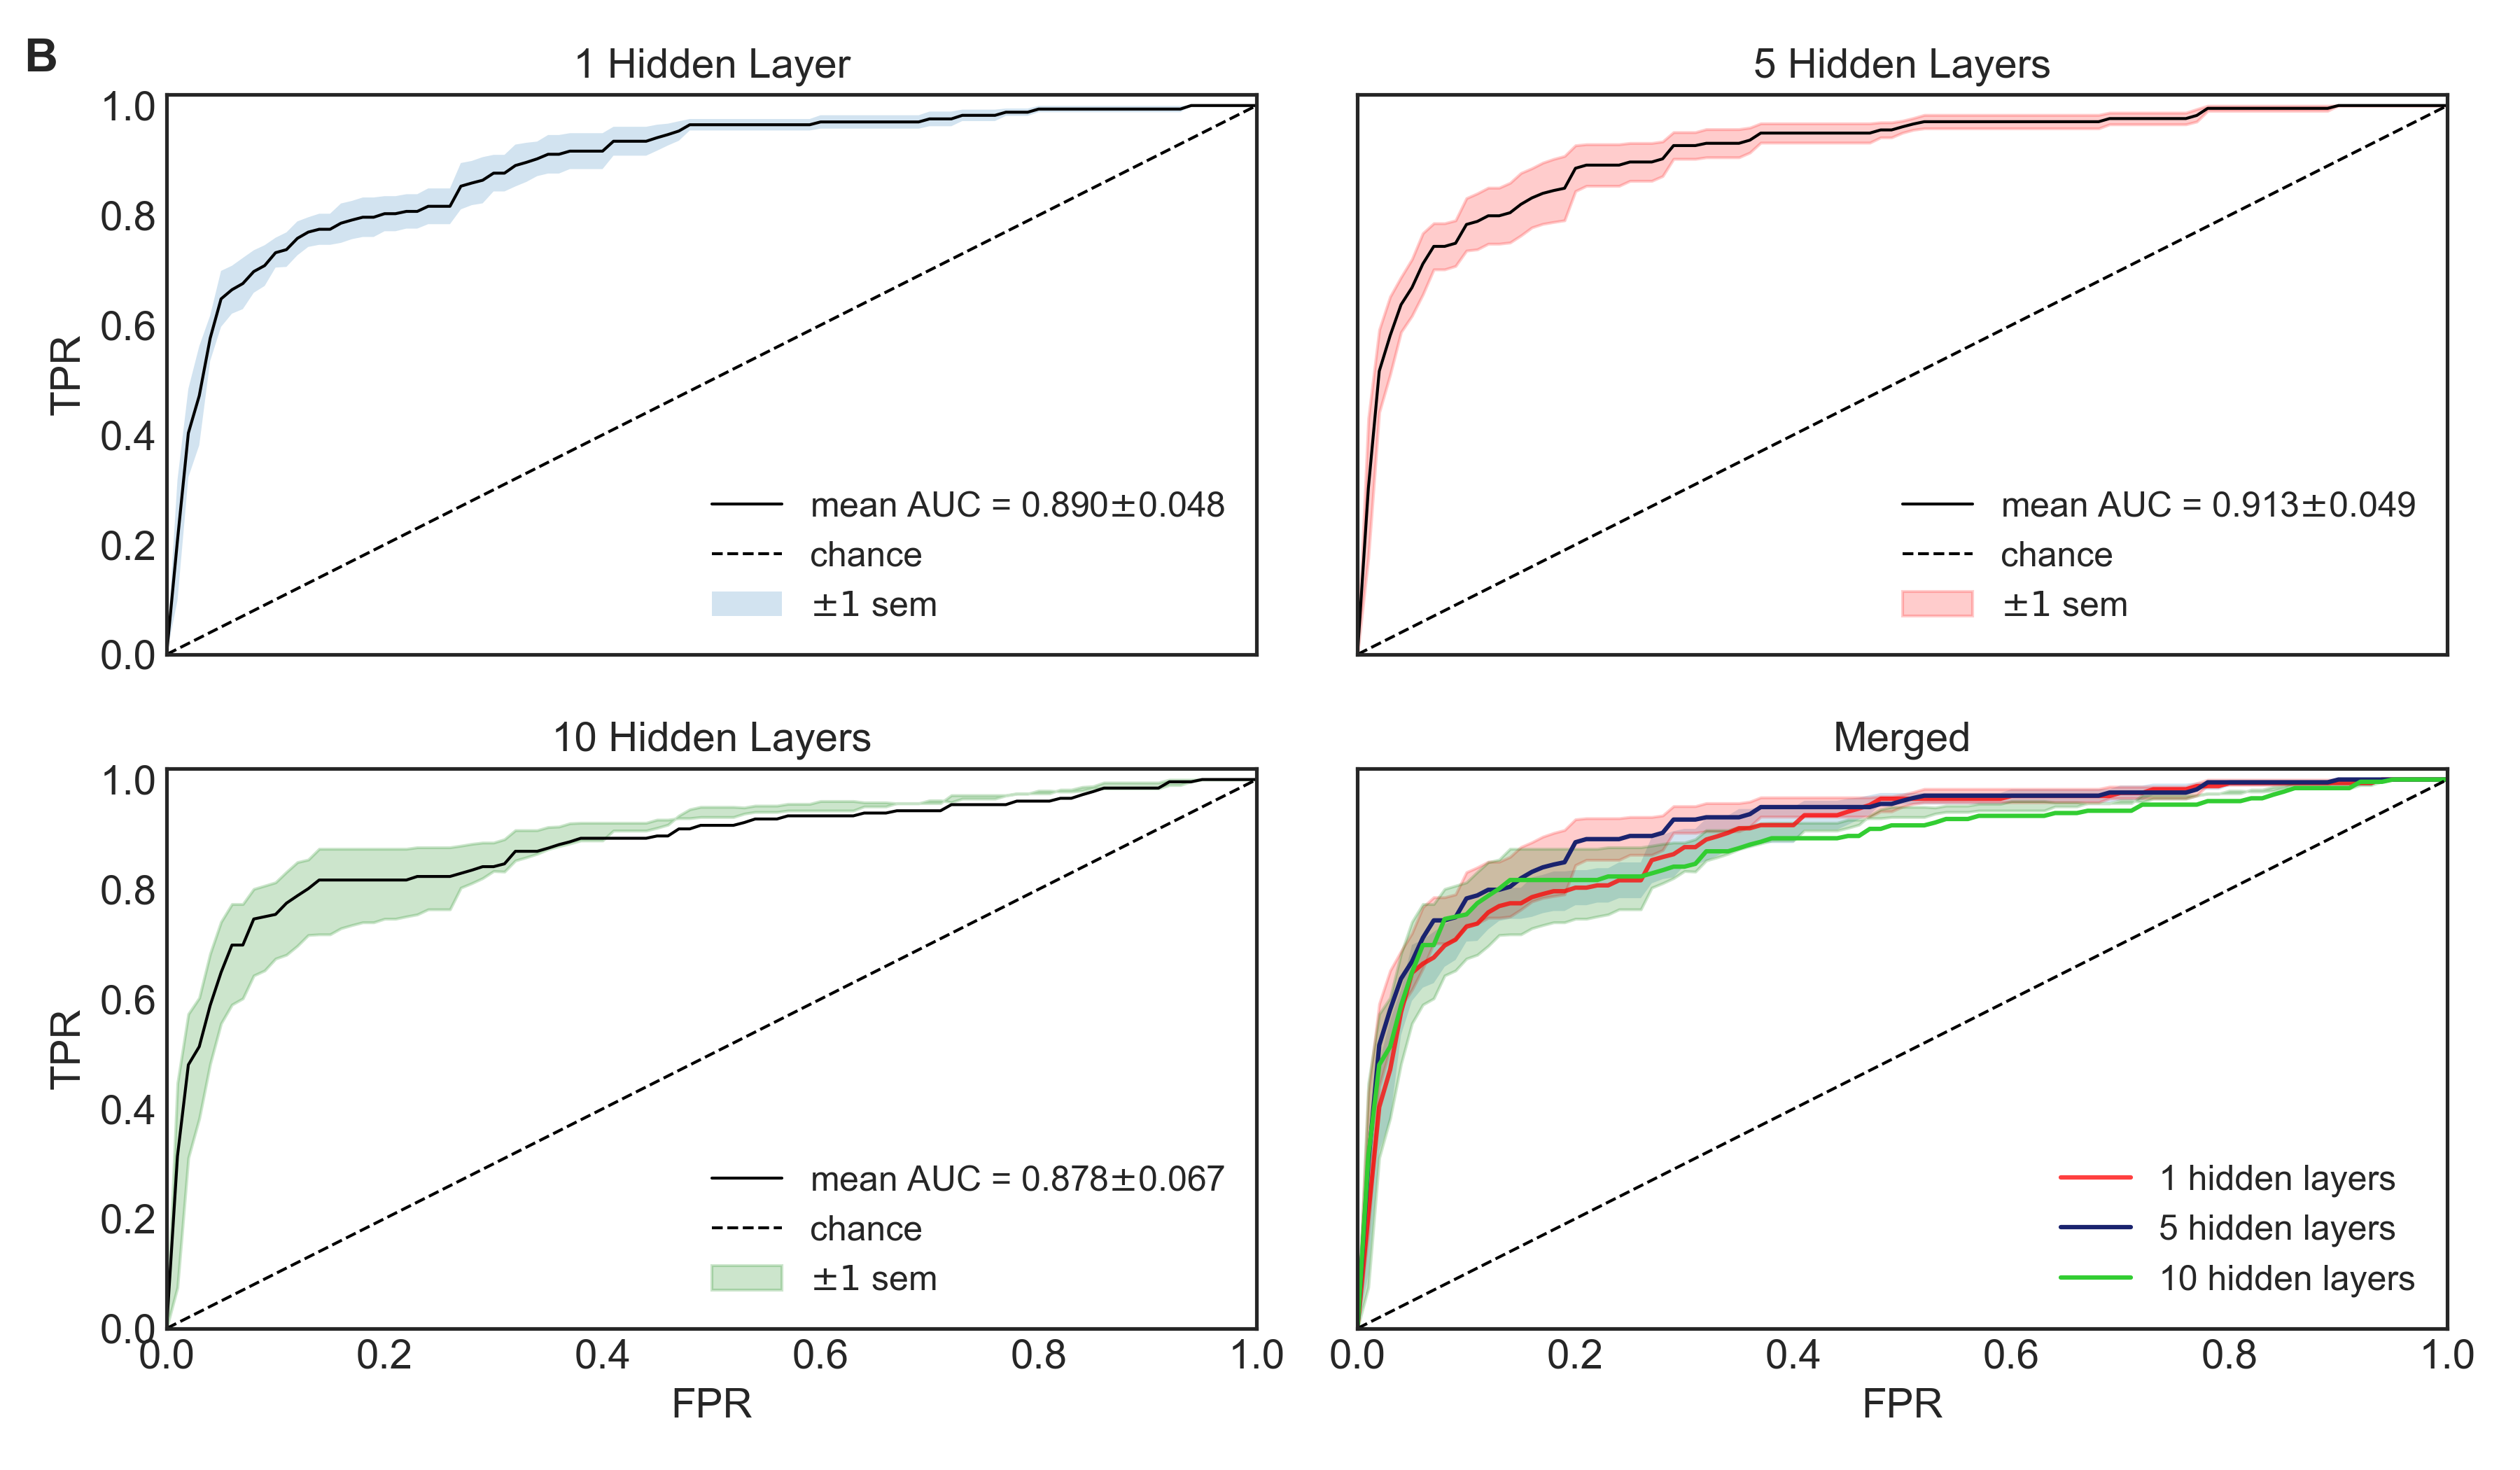
\includegraphics[width=\textwidth]{Figures/roc/roc_combined.png}
    \end{subfigure}

    \caption{(\textbf{A}) Confusion matrices for the 1, 5, and 10 hidden layer neural network models (the 15 hidden layer neural network is not shown). The models classify cell line microarray datasets into chemotherapy response cohorts. (\textbf{B}) ROC curves for 1, 5, and 10 hidden layers neural network models with confidence bands of $\pm 1$ standard error of the mean (sem). Each model was subject to 5-fold cross-validation, and the mean ROC curve across all trials was plotted.}
    \label{fig:nnet}
\end{figure*}


\subsection{Classification of cell lines using an optimized neural network}
The neural network was constructed using the Tensorflow Keras sequential deep learning API \cite{keras} in Python 3. The model underwent multiple instances of optimization, beginning with the depth of the network (1, 5, 10, and 15 hidden layers were evaluated). The rectified linear unit (ReLu) was chosen as the neuronal activation function for input and hidden layers. The output layer used a sigmoid activation for binary classification of inputs (i.e., chemotherapeutic response groups). The neural network was rigorously monitored for overfitting on the training dataset. To minimize overfitting, we applied L2 kernel regularization ($\lambda=10^{-3}$), batch normalization, and dropout layers with a 0.3 dropout rate to each hidden layer.

The dataset was randomly segregated using the Pareto principle \cite{pareto} where we reserved 80\% of the data for training and the remaining 20\% for validation. Model selection was performed by hyperparameter tuning using a grid search followed by 5-fold cross-validation (Table \ref{tab:params}). We performed a grid search with 3-fold cross-validation on the training data (80\% of the dataset; 432 training samples, 541 overall) to determine the parameters which minimize the binary cross-entropy loss function. GridSearchCV from the scikit-learn library \cite{scikit-learn} was used as a means of iterating through multiple possibilities of epochs, batch size, neurons per hidden layer, L2 regularization penalty, optimizer, and kernel initializer to find the optimal model (Table \ref{tab:params}). To prevent class imbalance during training, we used the Synthetic Minority Oversampling Technique (SMOTE) from the imblearn package \cite{imblearn} for Python 3. Each model’s performance on the testing dataset was evaluated by the Area Under Curve (AUC) value of the receiver operating characteristic (ROC) curve.


% Results
\section{Results}

% gene annotation figure
\begin{figure*}[!ht]
	\centering
	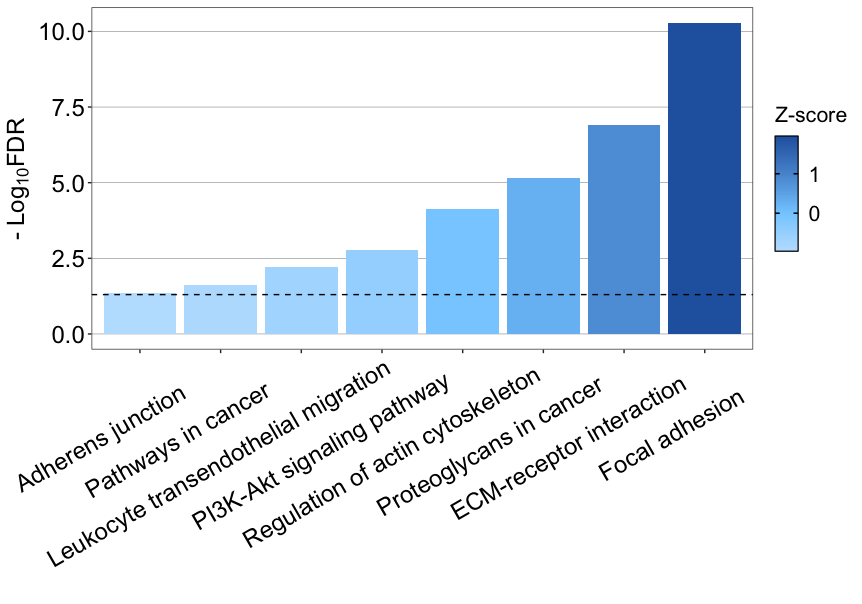
\includegraphics[width=\textwidth]{Figures/kegg.png}
	\caption{KEGG pathway functional enrichment for feature-selected genes included in the deep learning model. The vertical dotted line indicates the threshold for significance (adjusted $p < 0.05$).}
	\label{fig:kegg}
\end{figure*}

\subsection{Clustering of pan-cancer cell lines identifies two distinct therapeutic response cohorts}
From the GDSC consortium, we included 548 cell lines (49.4\% of the original cell lines) and 117 (46.6\% of the original drugs) chemotherapeutics for response group clustering. We assessed the ability of common molecular and clinical characteristics using principal component analysis (PCA) to stratify cell lines into groups with similar chemotherapeutic performance by subgrouping cell lines based upon these criteria.

To identify defined cohorts of pan-cancer cell lines with similar trends in therapeutic sensitivity, we employed unsupervised clustering of retained cell lines. PCA was used to reduce the dimensionality of the dataset, allowing for visualization of defined therapeutic response groups. This process identified two distinct clusters of therapeutic sensitivity (Fig. \ref{fig:clustering}), 362 cell lines identified in response group A, and 186 cell lines identified in response group B. That is, the cohorts perform substantially differently in a variety of therapeutics (Fig. \ref{fig:clustering}). To quantify differences in therapeutic response between these clusters, IC$_50$ values were compared between candidate cell lines (Fig. \ref{fig:clustering}). Of the 117 therapies included, 95 had significant differences in efficacy between the identified cohorts, suggesting that each represents groups of cell lines with vastly different therapeutic responses.


\subsection{Boruta selects 300 genes from the 16,382 gene dataset}
The Boruta algorithm was used to select genes that are estimated to have the greatest predictive contribution. The feature selection algorithm identified 300 relevant genes from the original set of 16,382 genes at $\alpha=0.05$ with a maximum tree depth of 5. To better understand the transcriptomic heterogeneity underlying the therapeutic response cohorts, a KEGG pathway enrichment analysis was performed on feature-selected genes used in the deep learning model. This analysis identified enrichment of gene sets associated with focal adhesion and PI3K signalling among others (Fig. \ref{fig:kegg}).


\subsection{A neural network with 10 hidden layers accurately classifies patients into responder and non-responder cohorts}
Unsupervised learning in the form of the k-means clustering of the cancer cell line transcriptomes indicated substantially different responses to chemotherapies. Using these distinct therapy response cohorts, we developed a deep learning binary classifier to predict drug response groups based on transcriptome data. We initially analyzed four neural network architectures, with 1, 5, 10, and 15 hidden layers (Fig. \ref{fig:neural_vis}). Hyperparameter optimization via grid search returned similar results for each model: 25 epochs, batch size of 16, 100 neurons per hidden layer, L2 kernel regularization with $\lambda=10^{-3}$, stochastic gradient descent as the optimizer, and a normal kernel initializer. Following this, we validated the various architectures with 5-fold cross-validation.

The neural network with 1 hidden layer performed poorly with 72.5\% accuracy. However, the 1 hidden layer model had the highest precision 97.8\% of the models (93.1\% for 5 hidden layers, 94.7\% for 10 hidden layers, 88.0\% for 15 hidden layers). The poor accuracy for the 1 hidden layer model was accounted for with a low negative predictive value (54.7\%; 86.1\% for 5 hidden layers, 97.0\% for 10 hidden layers, 100\% for 15 hidden layers). It was determined that the most accurate model was the neural network with 10 hidden layers (95.4\% accuracy; 72.5\% for 1 hidden layer, 90.8\% for 5 hidden layers, 90.8\% for 15 hidden layers).

An ROC curve was plotted for each of the neural network variants as an alternative evaluative method (Fig. \ref{fig:nnet}). The relative ratio between the model’s false positive rate and its true positive rate were averaged between 5 k-folds. The mean AUC for the 5 trials was used to compare the four network architectures. However, the differences between the various architectures for AUC was not significantly different. Consequently, confusion matrices (Fig. \ref{fig:nnet}) and associated misclassification rates were used to pick the optimal model. The neural net with 10 hidden layers demonstrated the best performance overall with a 95.4\% accuracy.


% Discussion
\section{Discussion}
It is well known that there is substantial heterogeneity concerning chemotherapeutic response between and among cancer types \cite{hetero, plasticity}. Although there have been multiple attempts to identify molecular and clinical features predictive of response to particular targeted therapies, there remains considerable variability within subgroups identified using these factors. In this study, we attempt to accurately cluster cancer cell lines into defined groups based on response to a large range of chemotherapeutics, and to create a deep learning transcriptomic model capable of accurately categorizing samples into these defined groups.

Using cell line chemotherapeutic efficacy obtained from the GDSC consortium, we employed unsupervised clustering techniques to identify two defined therapeutic response groups with significantly different responses to a multitude of standard chemotherapies. We demonstrate that commonly-used clinical criteria to predict chemotherapeutic performance -- such as anatomical location and morphologic subtype of cell lines, as well as TP53 and KRAS mutation status -- failed to identify defined clusters of cells with similar therapeutic responses (Fig. \ref{fig:overall_pca}). The consistent poor separability using these criteria and the relatively homogeneous distribution of cell responses to chemotherapeutics across major anatomical regions provides evidence for the utility of a pan-drug predictive biomarker. Given separability and the large feature space of the microarray data, a neural network was developed to classify cell lines into therapeutic response groups. This model may inform clinicians and researchers of the predicted therapeutic response of their patients to various chemotherapies.

Following the determination of two defined chemotherapeutic groups based on the GDSC dataset, we used a biologically agnostic feature selection algorithm, Boruta, to reduce the original set of 16,382 genes to a subset of 300 genes and to limiting preliminary bias due to multicollinearity in the model. The genes were then fed into neural networks, which were optimized using a grid search (Table \ref{tab:params}). Each network was carefully monitored for overfitting during training (loss value observed to decrease during training across all models). To minimize overfitting, we applied L2 kernel regularization ($\lambda=10^{-3}$), batch normalization, and dropout layers with a 0.3 dropout rate to each hidden layer. We determined from confusion matrices and ROC curve analysis that the best network architecture utilized 10 hidden layers, and demonstrated a 95.4\% accuracy in classifying response groups (Fig. \ref{fig:nnet}). This validates our postulate that gene expression is a prime determinant of chemotherapeutic response, and that cell lines of similar gene expression profile respond similarly to most chemotherapies.

The comparatively lower accuracy of the neural network with 1 hidden layer (72.5\%) suggests that the therapeutic response cohorts cannot be separated by a linear classifier and that classical machine learning techniques are insufficient to capture the complexity of the dataset. Furthermore, the decrease in accuracy from 10 hidden layers (95.4\%) to 15 hidden layers (90.8\%) indicates overfitting. To this end, a 10 hidden layer model is the ideal depth to analyze our data. Interestingly, there is no significant difference between the mean AUC for these models (Fig. \ref{fig:nnet}). Given that there were no significant differences between the mean AUC for these models, the confusion matrices were used to select the 10 hidden layer deep learning architecture as our model of choice.

The deep learning transcriptomic model consists of 300 genes, with KEGG pathway enrichment suggesting that predictive genes are associated with numerous pathways, most notably PI3K signalling and focal adhesion. Interestingly, there is a growing body of literature that suggests that PI3K/Akt pathway dysregulation may be associated with chemotherapeutic resistance in numerous different cancer and treatment contexts \cite{huang_2009}. Several studies have identified increases in Akt signalling in cancer cell lines exposed to chemotherapy and radiotherapy \cite{mapk, wort, phos}. Moreover, significant increases in Akt have been identified in chemoresistant and radioresistant cancer models \cite{cholangio}. Similarly, several studies have identified focal adhesion as a potential protective mechanism for various cancer cells. In fact, inhibition of particular integrin isoforms has been shown to increase the susceptibility of various cancer cell lines to conventional chemo/radiotherapies \cite{focal_adhesion}. Our results provide further evidence that dysregulation of PI3K signalling and focal adhesion may play a role in chemotherapy resistance in a pan-cancer context.

A major limitation of our study was the availability of large datasets to train our model. Here we faced a $p$ $\gg$ $n$ problem as machine learning models expect that the number of observations $n$ will be much larger than the number of features $p$. To minimize this bias, we applied the Boruta algorithm to reduce our 16,382 genes by 541 cell lines dataset to a 300 by 541 matrix. The algorithm has been shown in various studies to be an effective feature selection method in high dimensional omics datasets \cite{boruta}. To prevent overfitting of the reduced matrix, we applied L2 kernel regularization ($\lambda=10^{-3}$), batch normalization, and dropout layers (dropout rate of 0.3).

Future investigations will look to validate the predictive ability of the model to categorize chemotherapeutic response in various cancer types using the current transcriptomic signature. It is likely that the model accuracy will vary between therapy targets, and as such, further studies can make use of our project pipeline to create a stratified model whereby the drug class and target are additional inputs. In addition, biochemical features of gene targets may provide additional insights, especially for interpretability of the neural network output. It may also be interesting to select relevant genes using a different feature selector given that Boruta specifically operates on patterns of statistical relationships rather than biological relationships. Our use of Boruta was motivated by its efficacy demonstrated by prior studies of the algorithm as compared to other feature selectors \cite{boruta, deep_cell}. It is possible that a feature selection method informed by gene function and linkage disequilibrium could yield a different set of relevant genes.


% Conclusions
\section{Conclusions}
Using transcriptomic data from pan-cancer cell lines, two chemotherapeutic response clusters were identified via unsupervised learning in the form of k-means clustering. A feature selection algorithm was used to select a 300 gene subset which served as inputs to multiple neural networks. We determined that the network with 4 hidden layers was the most accurate model, producing a binary classifier to predict cell line therapy response with 91.7\% accuracy. Future studies will investigate the efficacy of our model to predict chemotherapy response in various cancer types and treatment contexts.


% Acknowledgements
\section*{Acknowledgements}
We wish to acknowledge the STEM Fellowship for organizing the 2020 Big Data Challenge, as well as Roche, SAS, Canadian Science Publishing, Digital Science, Altmetric, and Overleaf for their contributions that enabled this competition. We would like to thank our mentor, Dr. Daiva Nielsen for her feedback on our paper. We would also like to acknowledge Matthew Pietrosanu for his inputs.


\bibliography{bibliography}

\end{multicols*}



\clearpage

\section*{Supplementary Data}
\subsection*{Figures}
\begin{figure*}[!ht]
    \centering
    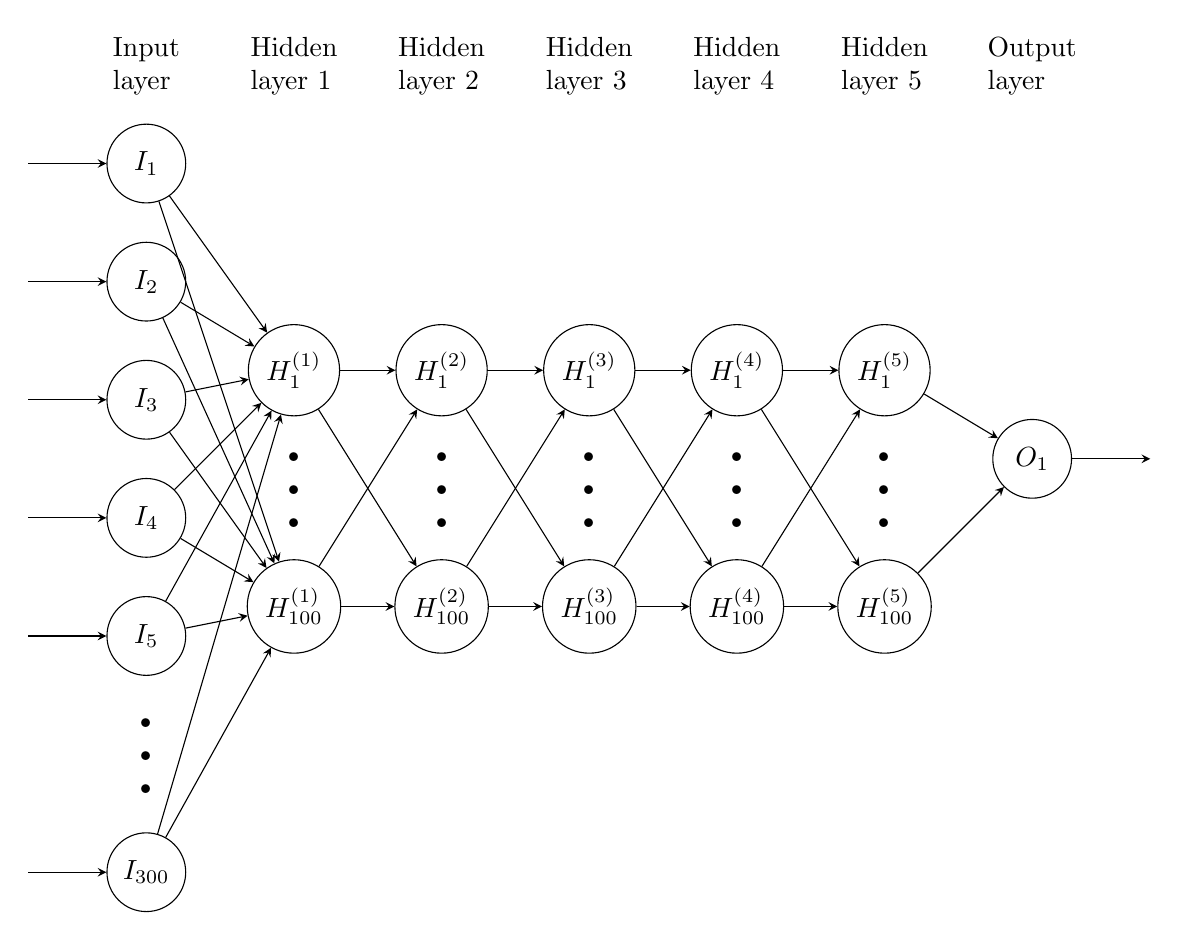
\begin{tikzpicture}[x=1.5cm, y=1.5cm, >=stealth]
    
        % nodes
        \foreach \m/\l [count=\y] in {1,2,3,4,5,missing,300}
            \node [every neuron/.try, neuron \m/.try] (input-\m) at (0,-\y) {\lmao{\l}};
        
        \foreach \m/\l [count=\y] in {1,missing,100}
            \node [every neuron/.try, neuron \m/.try] (hidden-\m) at (1.25,-1.75-\y) {\foo{\l}};

        \foreach \m/\l [count=\y] in {1,missing,100}
            \node [every neuron/.try, neuron \m/.try] (hidden1-\m) at (2.5,-1.75-\y) {\hehe{\l}};
    
        \foreach \m/\l [count=\y] in {1,missing,100}
            \node [every neuron/.try, neuron \m/.try] (hidden2-\m) at (3.75,-1.75-\y) {\hehetwo{\l}};
    
        \foreach \m/\l [count=\y] in {1,missing,100}
            \node [every neuron/.try, neuron \m/.try] (hidden3-\m) at (5,-1.75-\y) {\hehethree{\l}};
            	
        \foreach \m/\l [count=\y] in {1,missing,100}
			\node [every neuron/.try, neuron \m/.try] (hidden4-\m) at (6.25,-1.75-\y) {\hehefour{\l}};
    
        \foreach \m/\l [count=\y] in {1}
            \node [every neuron/.try, neuron \m/.try] (output-\m) at (7.5,0-2.5-\y) {$O_1$};

        % arrows
        \foreach \l [count=\i] in {1,2,3,4,5,300}
            \draw [<-] (input-\l) -- ++(-1,0) node [above, midway] {};
    
    	% input to hidden 1
        \foreach \l [count=\i] in {1,2,3,4,5,300}
            \foreach \k [count=\j] in {1,100}
              \draw [->] (input-\l) -- (hidden-\k);
   
    	% hidden 1 to hidden 2
        \foreach \l [count=\i] in {1,100}
            \foreach \k [count=\j] in {1,100}
              \draw [->] (hidden-\l) -- (hidden1-\k);
    
    	% hidden 2 to hidden 3
        \foreach \l [count=\i] in {1,100}
            \foreach \k [count=\j] in {1,100}
              \draw [->] (hidden1-\l) -- (hidden2-\k);
    
    	% hidden 3 to hidden 4
        \foreach \l [count=\i] in {1,100}
            \foreach \k [count=\j] in {1,100}
              \draw [->] (hidden2-\l) -- (hidden3-\k);
              
    	% hidden 4 to hidden 5
		\foreach \l [count=\i] in {1,100}
		\foreach \k [count=\j] in {1,100}
		\draw [->] (hidden3-\l) -- (hidden4-\k);
    
    	% hidden 5 to output
        \foreach \l [count=\i] in {1,100}
            \foreach \k [count=\j] in {1}
              \draw [->] (hidden4-\l) -- (output-\k);

        \foreach \l [count=\i] in {1}
            \draw [->] (output-\l) -- ++(+1,0) node [above, midway] {};

        % labelling layers
        \foreach \l [count=\x from 0] in {Input\\layer, Hidden\\layer 1, Hidden\\layer 2, Hidden\\layer 3, Hidden\\layer 4, Hidden\\layer 5, Output\\layer}
            \node [align=left, above] at (\x*1.25, -0.5) {\l};

    \end{tikzpicture}
    \caption{Neural network architecture representation with 5 hidden layers (300 inputs). Inputs include the feature-selected genes from the cell line microarray dataset. Each hidden layer has an L2 kernel regularization ($\lambda=10^{-3}$) and a dropout rate of 0.3. All hidden layers are subject to batch normalization.}
    \label{fig:neural_vis}
\end{figure*}


\subsection*{Tables}
\begin{table*}[!ht]
    \caption{Grid search parameters to optimize all implemented neural network architectures (1, 5, 10, and 15 hidden layers). Each grid search underwent 3-fold cross-validation on the training data. Optimal parameters: 25 epochs, batch size of 16, 100 neurons, $\lambda=10^{-3}$, stochastic gradient descent (sgd) as optimizer, normal kernel initializer.}
    \centering
    \label{tab:params}
    \begin{tabular}{l l l l l l}
        \toprule
        Epochs & Batches & Neurons & $\lambda$ (L2 reg) & Optimizer & Kernel initializer \\
        \midrule
        25 & 16 & 100 & 1e-4 & Sgd & Normal \\
        50 & 32 & 200 & 1e-3 & Adagrad & Uniform \\
        75 & 64 & 300 & 1e-2 & Adam & Glorot uniform \\
        \bottomrule
    \end{tabular}
\end{table*}


\end{document}















